\documentclass[11pt]{article}

\usepackage[utf8]{inputenc}
\usepackage[T1]{fontenc}
\usepackage[spanish,es-tabla]{babel}
\usepackage{lmodern}
\usepackage[a4paper,margin=2.2cm]{geometry}
\usepackage{graphicx}
\usepackage{float}
\usepackage{xcolor}
\usepackage{array}
\usepackage{longtable}
\usepackage{booktabs}
\usepackage{enumitem}
\usepackage{listings}
\usepackage{hyperref}

\graphicspath{{capturas/}}
\setlength{\parskip}{0.5em}
\setlength{\parindent}{0pt}
\renewcommand{\arraystretch}{1.3}
\definecolor{marca}{HTML}{0B3A5C}
\hypersetup{colorlinks=true,linkcolor=marca,urlcolor=marca}

\newcommand{\urlapp}{https://thankstochatgpt.github.io/LOARD}
\newcommand{\app}[1]{\href{\urlapp#1}{\texttt{#1}}}
\newcommand{\commit}[1]{\href{https://github.com/ThanksToChatGPT/LOARD/commit/#1}{\texttt{#1}}}

% Los prompts se pegan tal cual se escribieron.
\lstnewenvironment{prompt}{\lstset{
  basicstyle=\footnotesize\ttfamily,
  columns=fullflexible,
  keepspaces=true,
  breaklines=true,
  breakindent=0pt,
  breakatwhitespace=true,
  frame=single,
  framesep=3mm,
  xleftmargin=3mm,
  xrightmargin=3mm,
  rulecolor=\color{black!40},
  showstringspaces=false,
  literate={á}{{\'a}}1 {é}{{\'e}}1 {í}{{\'i}}1 {ó}{{\'o}}1 {ú}{{\'u}}1
           {Á}{{\'A}}1 {É}{{\'E}}1 {Í}{{\'I}}1 {Ó}{{\'O}}1 {Ú}{{\'U}}1
           {ñ}{{\~n}}1 {Ñ}{{\~N}}1 {¿}{{?`}}1 {¡}{{!`}}1
           {`}{{\textasciigrave}}1
}}{}

\newcommand{\captura}[3][0.65\linewidth]{%
  \begin{figure}[H]
    \centering
    \includegraphics[width=#1,height=0.45\textheight,keepaspectratio]{#2}
    \caption{#3}
  \end{figure}}

% Tabla de tres columnas para decisiones y ajustes.
\newenvironment{ajustes}[3]
  {\small\begin{longtable}{>{\raggedright\arraybackslash}p{4.5cm} >{\raggedright\arraybackslash}p{4.4cm} >{\raggedright\arraybackslash}p{6.4cm}}
   \toprule \textbf{#1} & \textbf{#2} & \textbf{#3} \\ \midrule \endhead
   \bottomrule \endfoot}
  {\end{longtable}\normalsize}

\title{Creación del prototipo: Uso de IA\\[0.3em]
\large Loard - Hito 2 - Módulo I: Prototipo}
\author{}
\date{}

\begin{document}
\maketitle

\section{Introducción}

El primer planteamiento fue usar v0 para crear los prototipos. Al usarlo vimos que solo genera código en React (Next.js) con Tailwind y no se lograron los resultados esperados, así que se decidió hacer el prototipo de alta fidelidad directamente en código, con las IA personales de cada integrante. El resultado está publicado en \href{\urlapp/}{\nolinkurl{https://thankstochatgpt.github.io/LOARD/}}.

Cada paso de este documento sigue el mismo flujo:

\begin{center}
\textbf{Prompt inicial $\rightarrow$ Resultado de la IA $\rightarrow$ Refactorización humana}
\end{center}

Los prompts se pegan tal cual se escribieron. En la refactorización humana nos enfocamos en lo que cambió para quien usa la aplicación: cómo se ve, qué tan fácil es de entender y qué tan cómodo es de usar.

\begin{center}
\begin{tabular}{>{\raggedright\arraybackslash}p{4.4cm} >{\raggedright\arraybackslash}p{3.8cm} >{\raggedright\arraybackslash}p{3.2cm} >{\raggedright\arraybackslash}p{3.4cm}}
\toprule
\textbf{Parte} & \textbf{Integrante} & \textbf{Herramienta} & \textbf{Sección} \\ \midrule
Sistema de diseño & Juan David Peña y Jonathan López & Claude & \ref{sec:paso1} y \ref{sec:paso2} \\
HU-M01 y HU-M02 & Juan David Peña & Codex & \ref{sec:hu01} \\
HU-M03 y HU-M04 & Sebastián Gutiérrez & Claude & \ref{sec:hu03} \\
HU-M05 y HU-M06 & Angel Inyena Pasuy & --- & \ref{sec:hu05} \\
HU-M07 y HU-M08 & Juan David Peña & Codex & \ref{sec:hu07} \\
HU-M09 y HU-M10 & Jonathan López & Claude & \ref{sec:hu09} y \ref{sec:hu10} \\
HU-M11 y HU-M12 & Ronald Chávez & ChatGPT & \ref{sec:hu11} \\
\bottomrule
\end{tabular}
\end{center}

% =====================================================================
\section{Paso 1: creación del sistema de diseño}\label{sec:paso1}

\subsection{Prompt}

Juan David Peña Lozada creó la primera versión de \texttt{design.md}, el documento que define cómo se ve la aplicación. El prompt original no quedó guardado, así que se describe el resultado.

\subsection{Resultado de la IA}

La primera versión proponía una estética ``sobria, de ingeniería industrial'': una paleta de azul pizarra con grises, y el color reservado para los estados (verde para lo aprobado o habilitado, ámbar para las alertas y rojo para los bloqueos). También definía un tema claro y uno oscuro.

\subsection{Refactorización humana}

Esa versión fue la base del Paso 2, donde se ajustó para el uso real en obra.

% =====================================================================
\section{Paso 2: refinamiento del sistema de diseño}\label{sec:paso2}

\subsection{Por qué se refinó}

La primera versión no servía del todo para el uso real en obra. El profesor
explicó que ``el color gris es el más fácil para buscar contrastes'', así que se
pidió una paleta sin grises (se escogió una paleta basada en azul petróleo). Loard se usa con sol directo, celulares de gama
baja y guantes, por lo que se subió el contraste y se pidieron botones más
grandes y separados. El recuadro que marca dónde está el teclado casi no se veía en modo oscuro, y las
animaciones muy rápidas se sentían como un salto brusco. Como la bitácora no se puede
borrar, un toque equivocado dejaba un registro falso; los 5 segundos de
``Deshacer'' dan tiempo de reaccionar. En frentes como Buenaventura puede no
haber señal hasta por 6 horas y el sistema no decía si el corte había salido.
Por último, como el equipo trabaja de manera asíncrona, hacía falta una sola
referencia de colores y componentes, una retícula común (12, 8 y 4
columnas, la vista en clase) y poder usar todo con el teclado.

\subsection{Prompt}

\begin{prompt}
Mejora `design.md` con estos cambios:

1. La paleta no usa grises para lograr contraste; propon otra paleta de colores.
2. Todo el texto tiene un contraste de 7:1.
3. El anillo de foco tiene un color para modo claro y otro para modo oscuro. El espacio entre el control y el anillo es del color del fondo.
4. Los botones miden 48 px en escritorio y 56 px en las pantallas móviles de corte e inspección SST. Entre controles hay 8 px.
5. Las transiciones duran 150 ms.
6. Antes de escribir en la bitácora aparece un aviso con "Deshacer" durante 5 segundos.
7. Los códigos de color solo aparecen en la sección 2. En el resto del documento cada color se llama por su nombre.
8. El documento explica qué pasa cuando se cae la señal.
9. El documento define la retícula.
10. Describe la navegacion por teclado
\end{prompt}

\subsection{Resultado de la IA}

La IA entregó el sistema de diseño refinado. Para poder ver todo junto se creó una página de muestra (\app{/muestra}) con los colores, la tipografía, la retícula y cada componente en sus estados.

\begin{figure}[H]
  \centering
  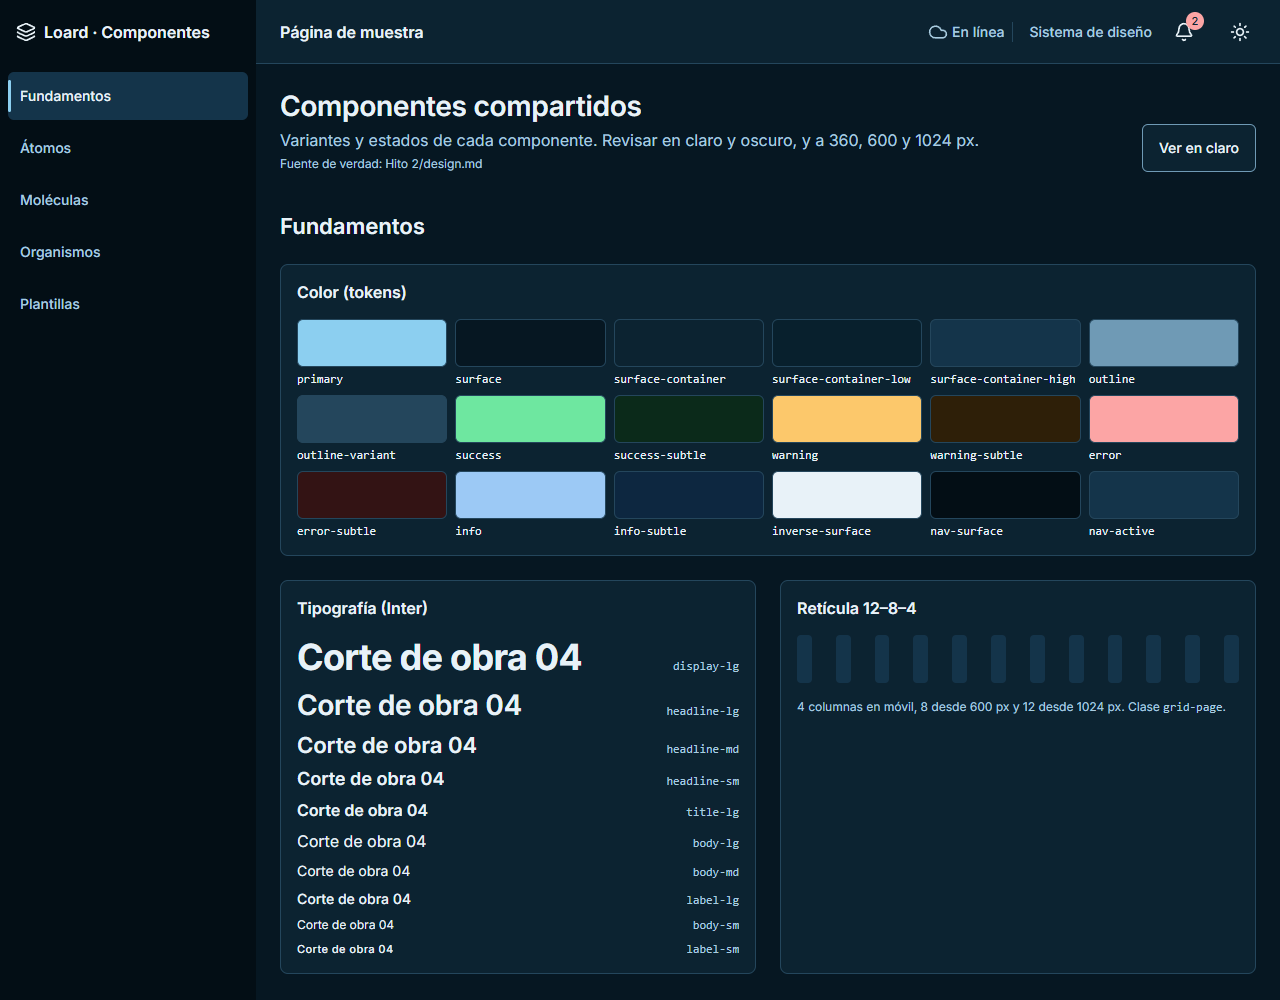
\includegraphics[width=0.5\linewidth]{muestra-1-fundamentos}\\[2mm]
  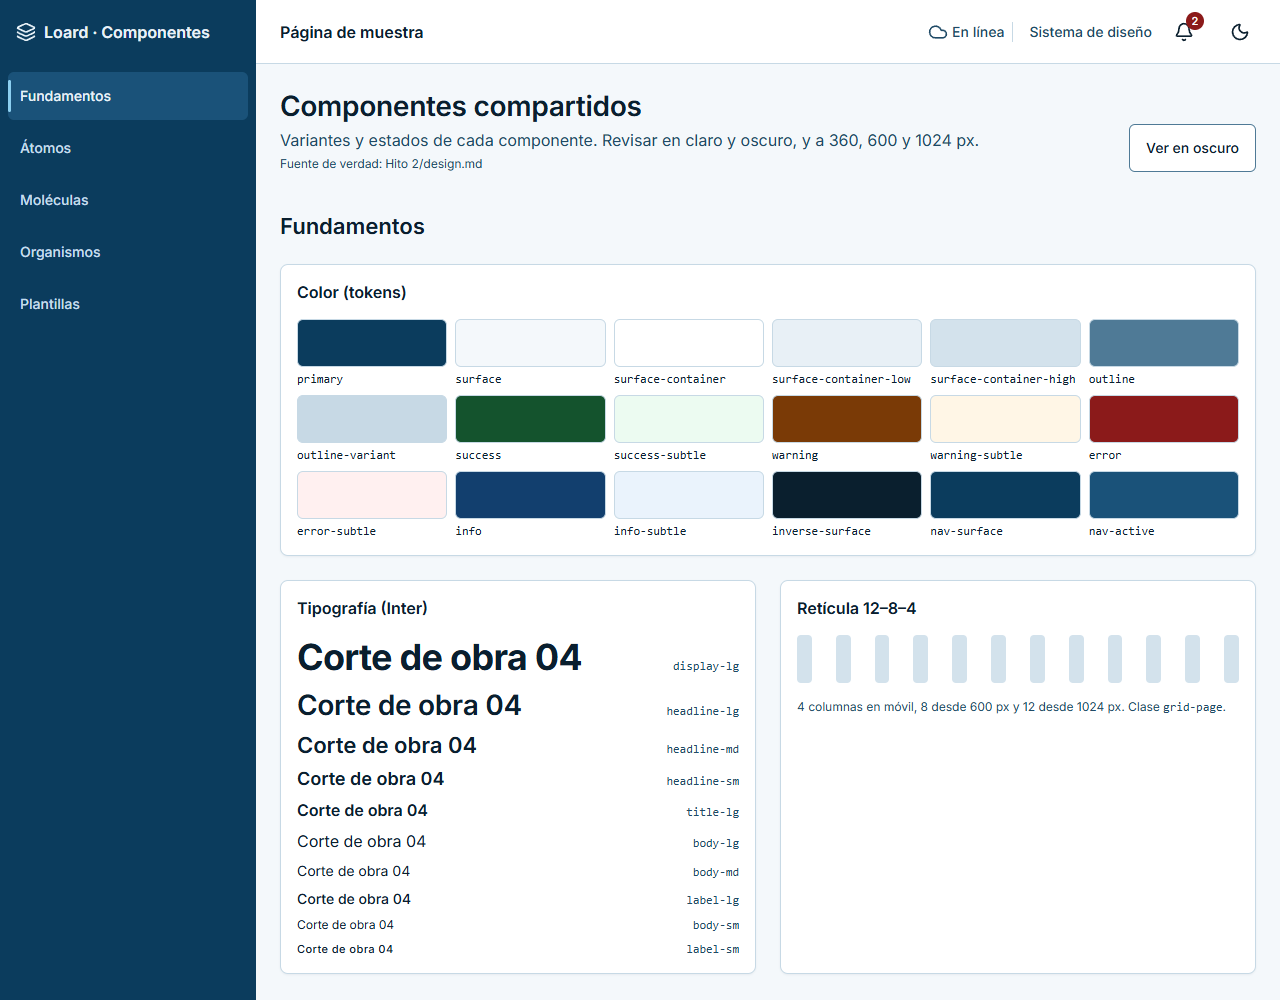
\includegraphics[width=0.5\linewidth]{muestra-5-claro}
  \caption{Página de muestra en modo oscuro (arriba) y claro (abajo): colores, tipografía y retícula.}
\end{figure}
\captura{muestra-2-atomos}{Botones, etiquetas de estado, casillas y barras de progreso.}
\captura{muestra-3-moleculas}{Campos, listas de selección, indicadores, avisos y carga de archivos.}
\captura{muestra-4-organismos}{Tablas, franja de conexión, avisos, carga de soportes y bitácora.}

\subsection{Refactorización humana}

Con la página de muestra a la vista se hicieron estos ajustes:

\begin{ajustes}{Qué se vio}{Ajuste}{Qué gana el usuario}
Los colores podían variar de una pantalla a otra. & Todos los colores salen de un solo lugar. & Cada estado se ve igual en toda la aplicación. \\
El recuadro del teclado se veía distinto según el fondo. & Se ajustó para que siempre tenga el mismo espacio alrededor del control. & Siempre se ve con claridad dónde está el teclado. \\
La letra se veía genérica para una herramienta de ingeniería. & Se cambió a IBM Plex Sans, incluida en la aplicación para que cargue sin señal. & Números y códigos más fáciles de leer en tablas. \\
\end{ajustes}

\subsection{Por qué importa elegir el diseño desde el inicio}

Tener el diseño escogido desde el principio permite que todo el equipo trabaje
en sintonía y adelanta trabajo de los módulos siguientes. De ahí en adelante, el
trabajo consiste solo en aplicar estos componentes, temas, colores y tipografías
a cada historia.

% =====================================================================
\section{HU-M01 y HU-M02: acceso y registro del corte}\label{sec:hu01}


\subsection{Prompt inicial}

El integrante aportó los archivos de guía y las referencias visuales. Pidió organizar bien el trabajo, reutilizar los componentes del equipo y guardar qué se editó. También aclaró que la entrega debía ser un prototipo y pidió dejar las credenciales de ejemplo completas al entrar. Algunas instrucciones reales:

\begin{prompt}
recuerda usar una buena estructura de carpetas re usar componentes etc..
\end{prompt}
\begin{prompt}
desactiva el backend por ahira y conviertelo en un prototipo de alta fidelidad de ejemplo
\end{prompt}
\begin{prompt}
no puedes poner esos datos de forma predeterminada cuando se entre a la app? osea la de correo y contraseña
\end{prompt}

\subsection{Resultado de la IA}

Codex construyó el acceso por perfiles (\app{/acceso}) y el registro y la edición de cortes (\app{/cortes}), con el diseño y los componentes del equipo.

\subsection{Refactorización humana}

\begin{ajustes}{Antes}{Decisión}{Qué gana el usuario}
Para entrar había que escribir correo y contraseña de memoria. & Al elegir un perfil, los datos de ejemplo aparecen completos. & Se entra con un clic, sin memorizar nada. \\
Al editar un corte se perdía lo anterior. & Cada edición guarda una versión nueva con autor, fecha y motivo. & Se puede consultar qué cambió, quién y por qué. \\
\end{ajustes}

\captura[0.8\linewidth]{corte-historial}{Historial de un corte: muestra las versiones y quién hizo el cambio.}

% =====================================================================
\section{HU-M03 y HU-M04: soportes y revisión del corte}\label{sec:hu03}


\subsection{Prompt inicial}

Se entregó a la IA la propuesta del MVP, la guía del Hito 2, el resumen de las heurísticas de Nielsen, este informe y el sistema de diseño. La instrucción fue:

\begin{prompt}
tengo que realizar el prototipo de la interfaz en dos historias de usuario ... basicamente tengo que entregar la Historia 3 y 4, para ello quisiera utilizar las 10 heuristicas de nielsen
\end{prompt}

Con esa instrucción la IA escribió primero una especificación con criterios, pantallas, casos de error y heurísticas. De ella salieron los prompts de cada historia:

\begin{prompt}
Haz el prototipo de la HU-03 en Hito 2/Modulo-I-Prototipo/prototipo, en src/features/cortes.
HU-03: como Ingeniero Residente quiero adjuntar fotografías y soportes en PDF al corte que
registré, para que lo reportado tenga evidencia y el director no tenga que pedírmela aparte.
Lee primero Hito 2/design.md (sobre todo 7.2, 8.3 y 6.1) y el README del módulo. Usa
FileUpload, UploadItem, Drawer y ToastProvider de @/components y las reglas de @/lib/archivos.
Lo que necesito:
* Sección "Soportes del corte" en el formulario y en el detalle del corte.
* Selección múltiple y arrastrar-soltar. Rechazo inmediato de tipo o peso con el mensaje de lib/archivos.
* Progreso simulado por archivo, "Confirmando carga..." y "Archivo cargado". Botón para cancelar.
* Si se pierde la conexión, el archivo queda en cola y se sube al volver.
* Visor lateral desde 1024 px y de pantalla completa en móvil. Al cerrar, el foco vuelve al soporte.
* Quitar un soporte con "Deshacer" de 5 s. En un corte Visado no se puede quitar ni agregar.
* El director ve los mismos soportes en modo consulta.
Agrega una foto y un PDF de ejemplo a los cortes de ejemplo.
\end{prompt}

\begin{prompt}
Haz el prototipo de la HU-04 en Hito 2/Modulo-I-Prototipo/prototipo, en src/features/cortes.
HU-04: como Director de Proyectos quiero revisar cada corte y visarlo o devolverlo con
observaciones puntuales, para asegurar que lo reportado es correcto sin frenar el frente.
Lee primero Hito 2/design.md (sobre todo 6.2B, 8.3 y 10) y el README del módulo. Usa Dialog,
Chip, Banner, Timeline y ToastProvider de @/components y los estados de @/lib/estados.
Lo que necesito:
* Para el director, /cortes abre filtrada en "En Revisión (Enviado)" con un KPI de pendientes.
* En el detalle, "Visar corte" con confirmación (foco inicial en Cancelar) y "Devolver con
  observaciones" con un diálogo: campo enfocado, chips de causas, mínimo 10 caracteres.
* Cada decisión crea una versión nueva con autor, rol, estado y observación en el historial.
* El residente ve la observación y puede corregir y reenviar. Registrar cortes nuevos nunca se bloquea.
* Sin conexión las acciones quedan deshabilitadas con el motivo. Si el corte cambió de versión, avisa.
El diálogo de devolución debe poder reutilizarse para "Observar requisito" del dossier.
\end{prompt}

\subsection{Resultado de la IA}

\begin{enumerate}
  \item \textbf{Especificación:} criterios, pantallas, casos de error y las 10 heurísticas. Ahí señaló una contradicción: el prototipo permitía editar un corte ya aprobado, y las historias lo prohíben.
  \item \textbf{HU-M03:} sección de soportes con barra de carga, espera cuando no hay señal, visor de fotos y PDF, y ``Deshacer'' al quitar un archivo.
  \item \textbf{HU-M04:} bandeja del Director, barra para visar o devolver, ventana de devolución con causas frecuentes y aviso para el residente.
\end{enumerate}

\subsection{Refactorización humana}

\begin{ajustes}{Problema}{Cambio}{Qué gana el usuario}
Se podía editar un corte ya visado. & El corte visado queda bloqueado y la pantalla explica por qué. & No se cambia por error algo ya aprobado. \\
En celular, la barra de revisión ocupaba casi media pantalla. & Solo los dos botones quedan fijos abajo; las explicaciones pasan al contenido. & El Director ve los datos que está revisando. \\
Después de visar o devolver, el teclado quedaba ``perdido'' en la página. & El foco pasa al nuevo estado del corte. & Quien usa teclado sabe de inmediato qué pasó. \\
``Cancelar'' se estiraba junto a un botón bloqueado. & Se alineó con el resto. & La ventana se ve ordenada. \\
``Devolver con observaciones'' se partía en dos líneas en pantallas grandes. & El botón mantiene su texto en una línea. & El botón se lee de un vistazo. \\
\end{ajustes}

\captura[0.8\linewidth]{revision-escritorio}{Detalle que revisa el Director, con la barra de decisión fija al pie.}

% =====================================================================
\section{HU-M05 y HU-M06: checklist y documentos del dossier}\label{sec:hu05}

Se construyó la checklist del dossier, los documentos del SIG y la carga de soportes, que después reutilizaron las demás pantallas del dossier, la bitácora y el tablero.

\begin{ajustes}{Pantalla}{Qué se ve}{Qué facilita}
Checklist del dossier (\app{/dossier}) & Seis carpetas con su avance y filtros por estado. & Ver de un vistazo qué falta en cada carpeta. \\
Detalle del requisito & Carga del soporte, validación con ``Deshacer'' y observación con causas. & Revisar sin salir de la checklist y corregir un error a tiempo. \\
Documentos del SIG (\app{/dossier/documentos}) & Búsqueda, versión vigente, historial y publicación de versiones nuevas. & Encontrar siempre el formato correcto. \\
\end{ajustes}

\captura[0.8\linewidth]{checklist-escritorio}{Checklist del dossier con el perfil Calidad.}

% =====================================================================
\section{HU-M07 y HU-M08: ensayos NDT y entrega del dossier}\label{sec:hu07}

Creado con las mismas indicaciones de la sección~\ref{sec:hu01}.

\subsection{Resultado de la IA}

Codex construyó el registro de ensayos NDT (\app{/dossier/ensayos}) y la pantalla de avance y entrega del dossier (\app{/dossier/avance}), conectadas con la checklist, la bitácora y el tablero del equipo.

\subsection{Refactorización humana}

\begin{ajustes}{Antes}{Decisión}{Qué gana el usuario}
Faltaba conectar los ensayos con el dossier. & Cada informe aparece como requisito en la carpeta que le corresponde. & Calidad revisa el ensayo en el mismo lugar que el resto del dossier. \\
El resultado ``Conforme'' del laboratorio se confundía con el documento aprobado. & Junto al resultado se aclara que el PDF debe ser revisado por Calidad. & Se distinguen los dos estados sin ayuda. \\
\end{ajustes}

% =====================================================================
\section{Prototipo de la HU-09 (Personal SST)}\label{sec:hu09}


\subsection{Prompt}

\begin{prompt}
Construye el prototipo de alta fidelidad de la Historia de usuario 9 en Hito 2/Modulo-I-Prototipo/prototipo, dentro de src/features/sst.
HU-09: como Coordinación SST quiero registrar los cursos normativos y la aptitud
médica de cada trabajador, con un semáforo de vencimiento a 30 y 15 días, para saber
a tiempo quién dejará de estar habilitado.
Antes de escribir, lee Hito 2/design.md y el README del Módulo I. Usa los componentes
de @/components y las reglas de @/lib (semaforo, estados, archivos).
Pantallas:

1. Lista de personal: indicadores por estado que filtran la tabla, búsqueda, y la
tabla ordenada con los críticos primero y el motivo visible en la fila.
2. Ficha del trabajador: cursos, aptitud médica e historial.
3. Formulario para registrar un curso, con carga del certificado y vista previa
del semáforo al elegir las fechas.
4. Formulario para actualizar la aptitud médica.

Reglas que no se pueden romper:

* La aptitud médica es solo Habilitado / No Habilitado con sus fechas. Ningún campo
de diagnóstico ni texto libre clínico.
* Sin conexión no se puede guardar; el botón queda bloqueado con el motivo.
* Los cursos no se editan ni se borran: se corrigen registrando uno nuevo.

Los datos de ejemplo van en src/features/sst, con fechas calculadas para
que se vean todos los estados del semáforo. Usa react router para conectar la pantalla en
App.tsx.
\end{prompt}

\subsection{Resultado de la IA}

La IA construyó las cuatro pantallas pedidas, disponibles en \app{/sst}.

\captura{sst-1-lista}{Lista de personal: indicadores por estado, búsqueda y tabla con los críticos primero.}
\captura{sst-2-ficha}{Ficha del trabajador: cursos, aptitud médica e historial.}
\captura{sst-3-curso}{Formulario para registrar un curso, con vista previa del semáforo y carga del certificado.}
\captura{sst-4-aptitud}{Formulario para actualizar la aptitud médica.}

\subsection{Refactorización humana}

\begin{ajustes}{Qué se vio}{Ajuste}{Qué gana el usuario}
Las pantallas SST tenían su propio marco, distinto al del resto. & Se usa el mismo menú y barra superior de toda la aplicación. & Moverse entre módulos se siente igual. \\
Los datos de los trabajadores solo los veía SST. & Se comparten con el registro del corte. & Lo que registra SST se refleja de inmediato al armar el corte. \\
\end{ajustes}

% =====================================================================
\section{Prototipo de la HU-10 (Personal del corte)}\label{sec:hu10}


\subsection{Prompt}

\begin{prompt}
Haz el prototipo de la HU-10 en Hito 2/Modulo-I-Prototipo/prototipo, en src/features/cortes.
HU-10: como Ingeniero Residente quiero que al agregar personal a un corte de obra no me
deje escoger trabajadores vencidos o No Habilitados, y que me diga por qué.
Lee primero design.md (sobre todo la 6.2A) y el README del módulo. Usa los componentes
de @/components y lo de @/lib. Los trabajadores y el semáforo ya están en features/sst,
reutilízalos (si toca moverlos a lib, muévelos).
Lo que necesito:

* Selector de personal con búsqueda. Salen todos, pero los bloqueados van abajo, en rojo,
con candado y el motivo (ej. "Bloqueado: Alturas vencido hace 4 días").
* Si intento seleccionar uno bloqueado, la fila se sacude y resalta el motivo. Tiene que
funcionar también con teclado.
* Sin internet usa los últimos datos SST y muestra a qué hora se actualizaron.
* Un resumen de los trabajadores escogidos con sus alertas de 15 y 30 días.

Conéctalo en App.tsx con react router
\end{prompt}

\subsection{Resultado de la IA}

La IA construyó el selector de personal, disponible en \app{/cortes/nuevo/personal}. En la captura hay cuatro trabajadores escogidos, con su resumen de alertas a la derecha, y se intentó marcar a un trabajador bloqueado (Jhon Angulo): la fila resalta el motivo y no se agrega.

\captura{cortes-2-seleccion}{Selector de personal del corte: disponibles arriba, bloqueados abajo con candado y motivo, y resumen con alertas de 15 y 30 días.}

\subsection{Refactorización humana}

\begin{ajustes}{Qué se vio}{Ajuste}{Qué gana el usuario}
Un trabajador bloqueado podía quedar marcado por un clic rápido. & La casilla de un bloqueado nunca se marca. & No se asigna personal sin habilitación. \\
La selección se perdía al recargar la página. & La selección se conserva. & No hay que volver a escoger a la cuadrilla. \\
El selector estaba en una pantalla aparte del corte. & Se integró al formulario del corte, con las horas de cada trabajador. & Todo el corte se llena en un solo lugar. \\
\end{ajustes}

% =====================================================================
\section{HU-M11 y HU-M12: bitácora y tablero}\label{sec:hu11}

Se construyeron la bitácora (\app{/dossier/bitacora}), que consulta Calidad, y el tablero del proyecto (\app{/dashboard}), que consultan Director y Gerencia.

\subsection{Prompt inicial}

Se utilizó ChatGPT como apoyo. La instrucción inicial fue desarrollar las HU-M11 y HU-M12, respetar el alcance actualizado y reutilizar el sistema de diseño del equipo.

\subsection{Resultado de la IA}

El resultado inicial incluyó las dos pantallas, la consulta por proyecto, los mensajes para cuando no hay datos o hay un error, y los cálculos del tablero.

\subsection{Refactorización humana}

\begin{ajustes}{Problema}{Cambio}{Qué gana el usuario}
Al elegir otro registro, la pantalla volvía a cargar desde cero. & Cambiar de registro es inmediato. & Se compara un registro con otro sin esperas. \\
``Actualizar'' dejaba la pantalla en blanco un momento. & Los datos siguen visibles y el botón dice ``Consultando''. & No se pierde de vista la información. \\
Las carpetas solo mostraban lo aprobado. & Cada carpeta muestra cuántos requisitos hay en cada estado. & Se ve qué falta, no solo qué está listo. \\
\end{ajustes}

\captura[0.8\linewidth]{bitacora-escritorio}{Bitácora del registro: cambios de un corte, el más reciente primero.}

\end{document}
